%%%%% Pedram Parsian %%%%%

\documentclass[twocolumn,a4paper]{report}

\usepackage[margin=0.25in]{geometry}
\usepackage{graphicx}
\usepackage{tikz}
\usepackage{pst-barcode}
%\usepackage{xepersian}
%\settextfont{IRLotus}


\title{گزارش نهایی کارت عضویت}
\author{پدرام پارسیان}

\begin{document}
\maketitle



\begin{figure}
\begin{center}
		
		\begin{tikzpicture}
		\node[inner sep=0] (img) at (0,0) {\fbox{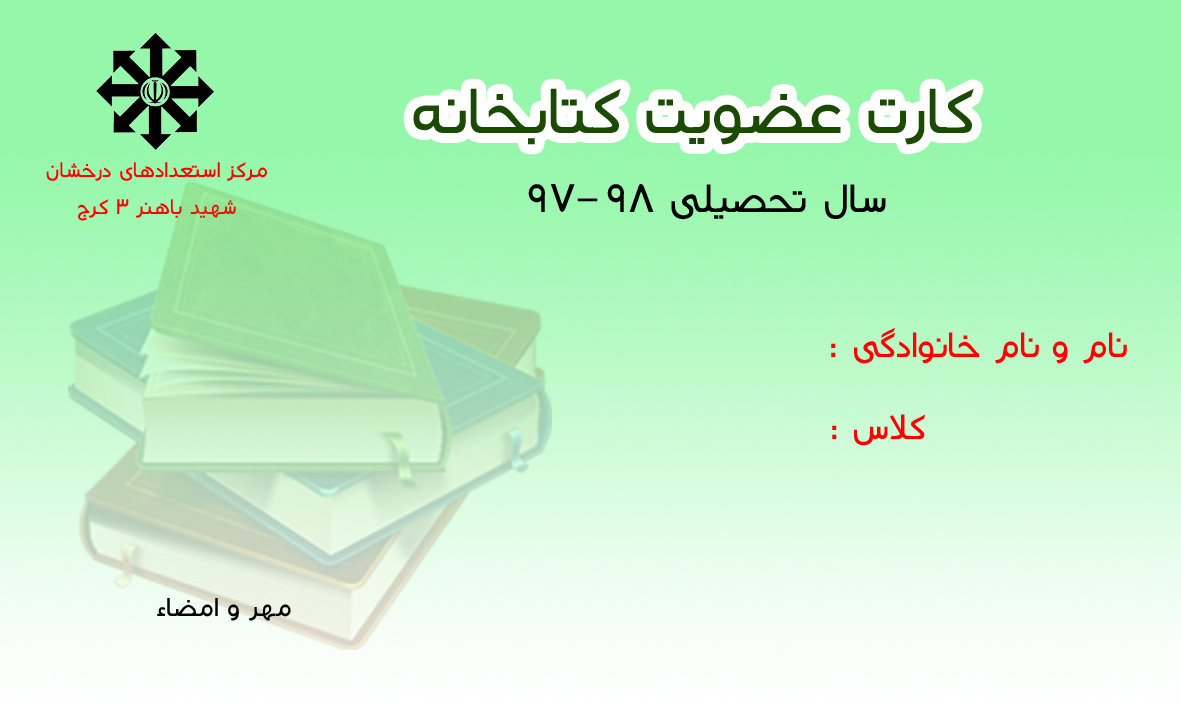
\includegraphics[height=5.7cm, keepaspectratio]{sample_card_template.jpg}}};
		\draw (0.15,0.08) node[text width=3cm, align=right] {Pedram Parsian};
		\draw (0.15,) node[below=1.35cm, text width=3cm, align=right] {7/1};
		\node[inner sep=0] (barcode) at (5,2.5) {
		 \begin{pspicture}
		\psbarcode{1234567890}{includetext height=0.5}{code128}
		\end{pspicture}};
		
		\end{tikzpicture}
		
		\vspace{0.5cm}
		
		\begin{tikzpicture}
		\node[inner sep=0] (img) at (0,0) {\fbox{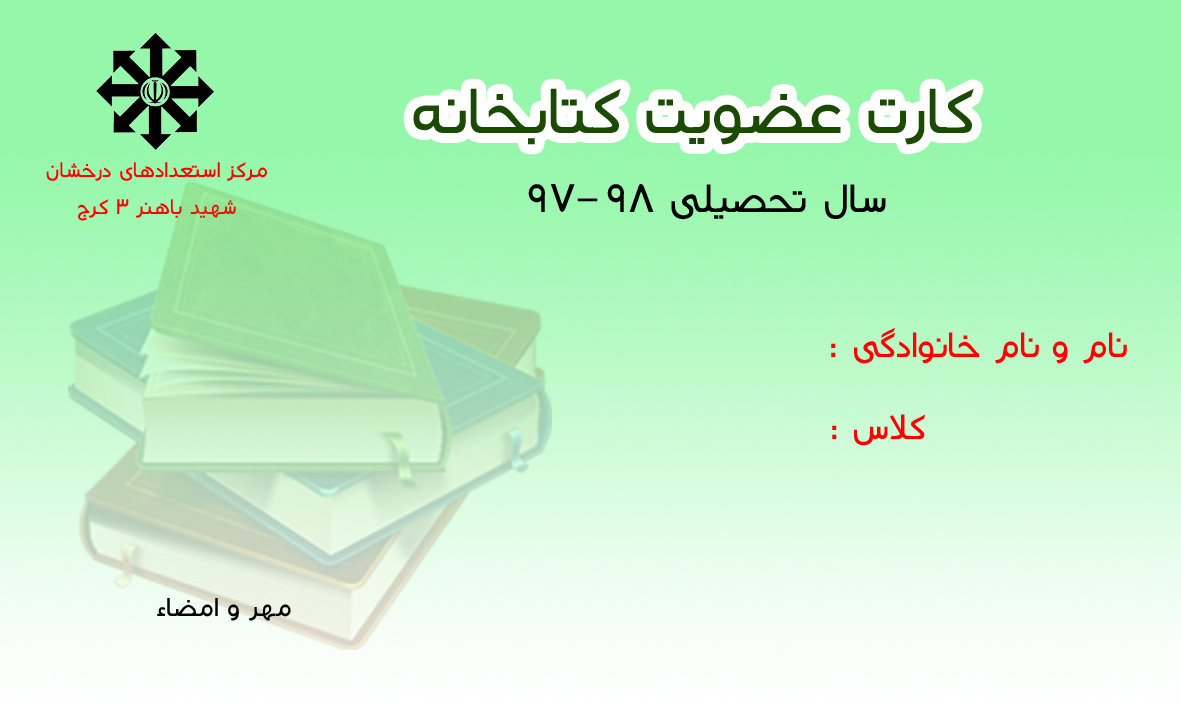
\includegraphics[height=5.7cm, keepaspectratio]{sample_card_template.jpg}}};
		\draw (0.15,0.08) node[text width=3cm, align=right] {Pedram Parsian};
		\draw (0.15,) node[below=1.35cm, text width=3cm, align=right] {7/1};
		\end{tikzpicture}
		
		\vspace{0.5cm}
		
		\begin{tikzpicture}
		\node[inner sep=0] (img) at (0,0) {\fbox{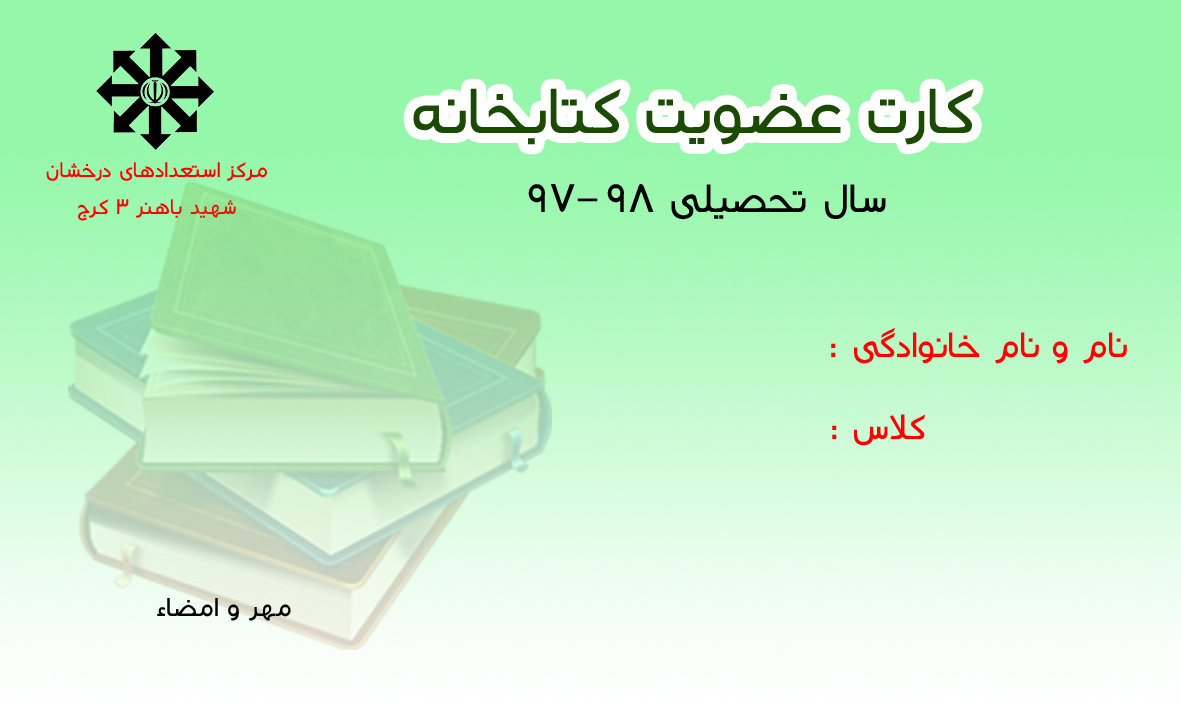
\includegraphics[height=5.7cm, keepaspectratio]{sample_card_template.jpg}}};
		\draw (0.15,0.08) node[text width=3cm, align=right] {Pedram Parsian};
		\draw (0.15,) node[below=1.35cm, text width=3cm, align=right] {7/1};
		\end{tikzpicture}
		
		\vspace{0.5cm}
		
		\begin{tikzpicture}
		\node[inner sep=0] (img) at (0,0) {\fbox{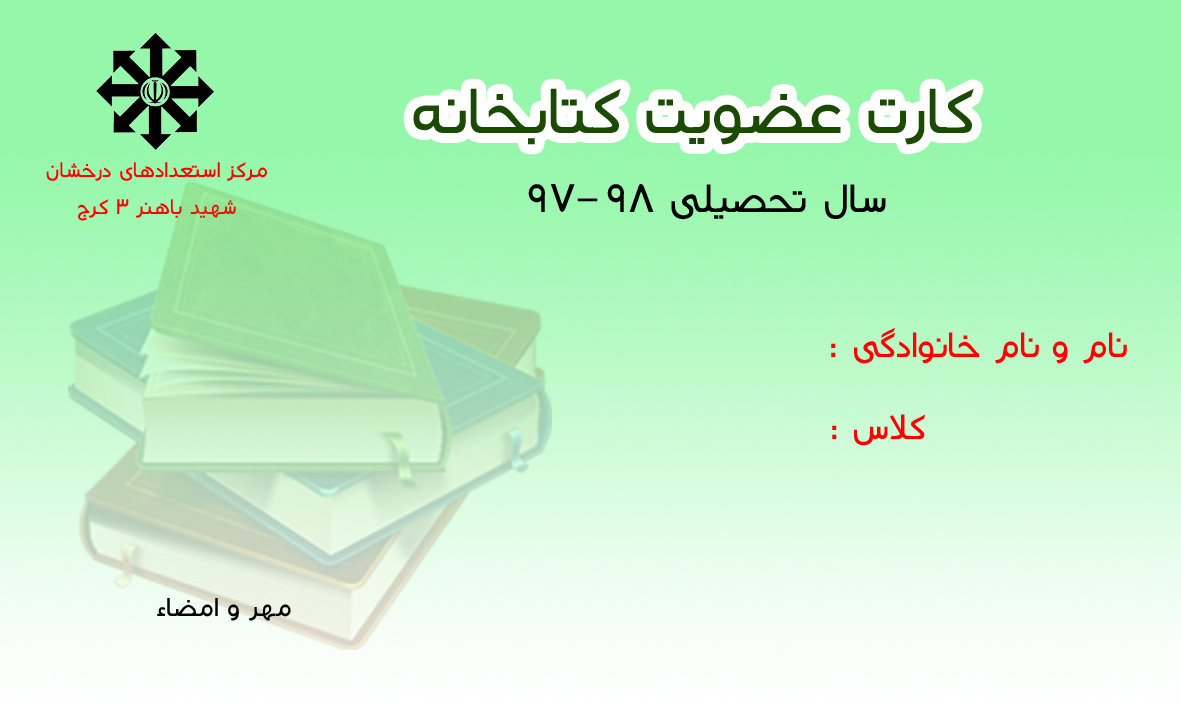
\includegraphics[height=5.7cm, keepaspectratio]{sample_card_template.jpg}}};
		\draw (0.15,0.08) node[text width=3cm, align=right] {Pedram Parsian};
		\draw (0.15,) node[below=1.35cm, text width=3cm, align=right] {7/1};
		\end{tikzpicture}

\end{center}
\end{figure}
%\end{tikzpicture}
\end{document}